
\section{Sample proofs for response properties}
\label{sec:results}
\subsection{Proof  1}
In this subsection, we want to prove $\RESP{n=1}{{n}=3}$ for Machine M0 below.\\

\usetikzlibrary{arrows}
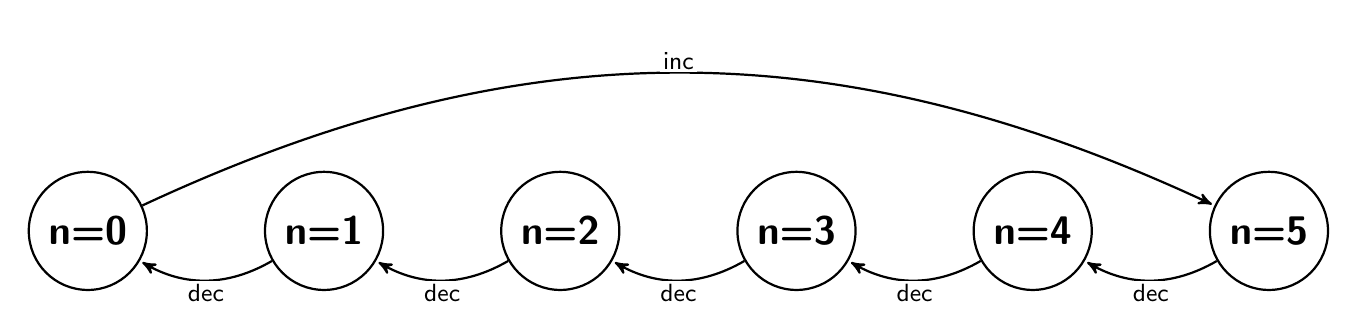
\begin{tikzpicture}[->,>=stealth',shorten >=1pt,auto,node distance=3cm,
  thick,main node/.style={circle,fill=white!20,draw,
  font=\sffamily\Large\bfseries,minimum size=15mm}]

  \node[main node] (A) {n=0};
  \node[main node] (B) [right of=A] {n=1};
  \node[main node] (C) [right of=B] {n=2};
  \node[main node] (D) [right of=C] {n=3};
  \node[main node] (E) [right of=D] {n=4};
  \node[main node] (F) [right of=E] {n=5};

  \path[every node/.style={font=\sffamily\small,
  		fill=white,inner sep=1pt}]
  	% Right-hand-side arrows rendered from top to bottom to
  	% achieve proper rendering of labels over arrows.
    (A) edge [bend left=25] node {inc} (F)
    (B) edge [bend left=30] node {dec} (A)
    (C) edge [bend left=30] node {dec} (B)
    (D) edge [bend left=30] node {dec} (C)
    (E) edge [bend left=30] node {dec} (D)
    (F) edge [bend left=30] node {dec} (E);
   
\end{tikzpicture}
\\\\
For machine M0, we know that:
\begin{gather*}
J = (n\in\mathbb{N})\\ 
I_1 = \{inc,dec\}\\
g_{inc} = \{n | n < 1\}, a_{inc} = (n' = n + 5), \mathrm{Only}({inc}) = \{n | n < 1\}\\
g_{dec} = \{n | n > 0\}, a_{dec} = (n' = n - 1), \mathrm{Only}({dec}) = \{n | n > 0\}\\
thm_{InfExe} : (n < 1\Or{n} > 0) 
\end{gather*} 
\paragraph{Infinite execution proof for M0}
Since ${J}\Equiv(n\in\mathbb{N})\Implies(n < 1\Or{n} > 0)\Equiv{thm_{InfExe}}$, $\mathrm{M0}$ have infinite execution.
\paragraph{Response proof for M0}
For proving $\RESP{n = 1}{n = 0}$ we have:
\begin{gather*}
   p = (n = 1), q = (n = 0)\\   
   (n = 1)\in\mathrm{Only}({dec})\Equiv\mathrm{Only_{dec}}(n = 1)
\end{gather*}
By applying to rule \texttt{$\mathrm{RESP_{ONLY}}$}, we have:
\begin{gather*}
  \mathrm{Only}_{dec}({n = 1})\\
  \frac{{J}\And{g_{dec}}\And{(n = 1)}\And{a_{dec}} = (n' = 0)}{\RESP{n = 1}{n = 0}}
\end{gather*}
Similarly, we can prove ${\RESP{n = 5}{n = 4}}$ and ${\RESP{n = 4}{n = 3}}$.\\
For proving $\RESP{n = 0}{n = 5}$ we have:
\begin{gather*}
   p = (n = 0), q = (n = 5)\\   
   (n = 0)\in\mathrm{Only}({inc})\Equiv\mathrm{Only_{inc}}(n = 0)
\end{gather*}
By applying to rule \texttt{$\mathrm{RESP_{ONLY}}$}, we have:
\begin{gather*}
  \mathrm{Only}_{inc}({n = 0})\\
  \frac{{J}\And{g_{inc}}\And{(n = 0)}\And{a_{inc}} = (n' = 5)}{\RESP{n = 0}{n = 5}}
\end{gather*}
Since we proved ${\RESP{n = 1}{n = 0}}$, ${\RESP{n = 0}{n = 5}}$, ${\RESP{n = 5}{n = 4}}$ and ${\RESP{n = 4}{n = 3}}$, by applying to the transitivity of response, we get $\RESP{n=1}{{n}=3}$.
Testing citations~\cite{Engelhardt2013, MannaPnueli1991:szym,
  HoangAbrial:ICFEM2011, MannaPnueli92, MannaPnueli:REX1988}.


\thispagestyle{empty}
\begin{description}
\MACHINE{M0}
\VARIABLES
	\begin{description}
		\Item{ n }
	\end{description}
\INVARIANTS
	\begin{description}
		\nItem{ inv1 }{ n \in  \nat }
		\nItem{ {\it thm\_InfExe} }{ n <  1 \lor  n >  0 }
	\end{description}
\EVENTS
	\INITIALISATION
		\begin{description}
		\BeginAct
			\begin{description}
			\nItem{ act1 }{ n :=  0 }
			\end{description}
		\EndAct
		\end{description}
	\EVT {inc}
		\begin{description}
		\WhenGrd
			\begin{description}
			\nItem{ grd1 }{ n <  1 }
			\end{description}
		\ThenAct
			\begin{description}
			\nItem{ act1 }{ n :=  n + 5 }
			\end{description}
		\EndAct
		\end{description}
	\EVT {dec}
		\begin{description}
		\WhenGrd
			\begin{description}
			\nItem{ grd1 }{ n >  0 }
			\end{description}
		\ThenAct
			\begin{description}
			\nItem{ act1 }{ n :=  n -  1 }
			\end{description}
		\EndAct
		\end{description}
\END
\end{description}
